\section{An Observed-Lens Baseline and Withheld-Light Test}
\label{sec:observed-lens}
\subsection{Data, calibration and reserved observations}
We next apply the transfer-to-identifiability question to HE~0435$-$1223,
selected for its resolved four-image geometry and public long-term
COSMOGRAIL monitoring~\cite{Bonvin2017,Millon2020COSMOGRAIL}.
The adopted redshifts are $z_l=0.4546$ and $z_s=1.693$.
HST point-image and galaxy astrometry comes from
Courbin et al.~\cite{Courbin2011}, with the required additional $2$ mas
systematic uncertainty. The unavailable full positional covariance is
approximated by a diagonal covariance for the published relative positions;
we do not fit Einstein-ring pixels or published cosmological posteriors.

The endpoint of the earlier 884-epoch release fixes the chronological
boundary at native day $57447.03918$. The 2020 release reprocesses some
historical photometry, so we use its single consistent reduction:
902 training epochs and 100 later epochs, each containing four R-band
magnitudes and their errors. The historical release is not concatenated
with the newer reduction. The catalogue and release page differ by half
a day in their stated absolute epoch origin; native day differences
suffice for all splits and delays here.
This is retrospective chronological validation in a common reduction,
not a prospectively blinded observing campaign.

The protocol was fixed before fitting. Variability, microlensing and
macro parameters were fitted on historical observations only, and the
prediction artifact was committed before target scoring. The primary test
conditions on all 100 later image-B observations as an explicitly allowed
driver and predicts the 300 reserved A/C/D magnitudes. It is a batch
cross-image conditional prediction; some driver observations are later
than a target date. A separate all-channel forecast reserves all 400 later
magnitudes and conditions on training data only. Neither test refits
parameters, photometric offsets or extrinsic curves against its targets.

\subsection{The conditional physical and brightness applications}
We retain the same fixed R1 reference calibration, recomputing its FLRW
distance maps and local scalar coefficients at the observed redshifts.
This common geometry defines the conventional galaxy-potential benchmark
and the conditional R1 comparison; it is not a cosmological viability fit.
The local body is a positive Plummer source with fitted mass and scale.
A rear quadratic optical screen at the fixed conditional redshift
$z_p=0.8$ supplies asymmetric propagation. It is total optical boundary
information, rather than an identified physical perturber or a solved
same-domain scalar environment.

For physical screen potential $\widehat\psi_p(x_p)=x_p^TUx_p/2$ with
symmetric $U$, the original two-plane ray equations are
\begin{align}
 x_p&=D_p\theta-D_{lp}\widehat\alpha_l(D_l\theta),\nonumber\\
 x_s&=D_s\theta-D_{ls}\widehat\alpha_l(D_l\theta)-D_{ps}Ux_p.
 \label{eq:observed-two-plane}
\end{align}
Their elimination gives the compatible maps
\begin{equation}
 \mathsf D_{ol}=D_lI,\qquad
 \mathsf D_{os}=D_sI-D_{ps}D_pU,\qquad
 \mathsf D_{ls}=D_{ls}I-D_{ps}D_{lp}U.
 \label{eq:observed-screen-maps}
\end{equation}
The same eliminated two-plane arrival action gives the time-delay matrix
and observer-clock normalization used in Equation~\eqref{eq:arrival}.
No second sheet is added to the local body. Supplementary Note S9 gives
the full action and Schur reduction, including the required pre-conjugate
map conditions and the isolated spherical scalar boundary prescription.

The local field is still the original regular sourced solution. At the
refitted R1 image-A impact $r=7.74161173$ kpc, the executed section has
$\pi'_T/(\Mpl H_0)=-1.83519726\times10^{-4}$ and consumed source
$J_{\rm eff}/(\Mpl H_0^2)=-40596.7951$.
In $H_0=\Mpl=1$ units the integrated scalar left and source
rows both give $-2.36867868266\times10^{-13}$; the corresponding metric
Gauss rows both give $5.16669407301\times10^{-12}$.
The maximum scalar-flux residual is $1.10\times10^{-15}$ and the four
metric-Gauss section residuals are below $3.80\times10^{-16}$ relative.
These numerical field residuals do not establish that the assumed galaxy
profile is observationally adequate.

For observed magnitude $m_{ik}$ at observer time $t_{ik}$, we apply the
classical variability likelihood
\begin{equation}
 m_{ik}=m_0+b_i+q(t_{ik}-d_i)+e_i(t_{ik})+\epsilon_{ik}.
 \label{eq:observed-brightness}
\end{equation}
Here $q$ is a common stationary Ornstein--Uhlenbeck process, a standard
empirical quasar-variability model~\cite{Kelly2009}; $e_i$ are independent
slower processes for extrinsic variability, and $b_i$ have proper broad
Gaussian offset priors. Their covariances are
$\sigma_q^2e^{-|\Delta t|/\tau_q}$ and
$\sigma_e^2e^{-|\Delta t|/\tau_e}$, respectively. Quoted photometric
variance plus fitted common jitter supplies the independent measurement
noise approximation; the total brightness covariance remains correlated.
This empirical likelihood does not replace a BHSM quantum-state kernel.

An exact nine-state Kalman filter evaluates the normalized likelihood.
At source time $u=t-d_i$, its state is
$(q,e_A,e_B,e_C,e_D,b_A,b_B,b_C,b_D)$, with OU transitions for the first
five components and constant offsets. Smoothing over each permitted conditioning set gives
predictive means and marginal variances. The joint test score is
\begin{equation}
 \log p(y_{\rm target}\mid y_{\rm condition},\widehat\vartheta)
 =\log p(y_{\rm condition},y_{\rm target}\mid\widehat\vartheta)
  -\log p(y_{\rm condition}\mid\widehat\vartheta),
 \label{eq:observed-score}
\end{equation}
with all parameters $\widehat\vartheta$ frozen. It is not the sum of
univariate marginal scores. Supplementary Note S10 derives these
applications and compares them with independent dense-Gaussian formulas.

The empirical training delays relative to A are
\[
 (d_B,d_C,d_D)=(6.41984,-0.97473,12.48799)\ {\rm days},
\]
where positive means later arrival. Four fixed starts retain multiple local modes; two reach
nearly the same best likelihood. Both fitted variability timescales hit
their preset upper bounds, $1500$ and $10000$ days. Delay-curvature
estimates depend materially on step size and are not calibrated confidence
limits. The macro fits use the exact historical brightness likelihood
after initialization. Their shared variability hyperparameters remain
fixed: this is a two-stage conditional empirical Bayes calculation,
rather than a fully marginalized physical and stochastic posterior.

\subsection{Frozen predictions and observed performance}
The conventional macro fit predicts delays
$(6.020014,0.672696,13.611423)$ days; the separately refitted R1 model
predicts $(6.022659,0.672780,13.616498)$ days.
Their astrometric residual sums are $12.714$ and $12.695$ over eight
relative-coordinate rows. The conventional fit has
$M=10^{11.61394}M_\odot$, Plummer scale $a=10^{0.70626}$ kpc and
screen convergence $0.3844$ within the declared bounds. This large
conditional propagation nuisance is not an independently measured
line-of-sight convergence.

Activating R1 at exactly the conventional fitted body, source and screen
changes the three delays by $(19.2903,0.9386,29.0367)$ s.
Separately refitted differences, approximately $(228.51,7.23,438.44)$ s,
also contain nuisance reallocation and optimizer termination effects;
they are not the fixed-body physical signal.
The independent full two-plane and compact actions agree to
$2.4\times10^{-14}$ day. A positive conventional effective mass still
reproduces the entire retained R1 transfer, and therefore its test score.
That shared score is a structural equality, not an independent empirical
confirmation.

\begin{table}[htbp]
 \centering
 \caption{Frozen later-B-conditioned predictions of 300 withheld A/C/D
 magnitudes. Log scores are joint continuous predictive densities in
 the same magnitude units. The zero-delay row keeps the same frozen
 variability parameters; it is a control, not a separately optimized
 alternative model. Intervals condition on point-fitted parameters.}
 \label{tab:observed-heldout}
 \begin{tabular}{lrrr}
 \toprule
 Transfer & Joint log score & RMSE (mag) & 95\% coverage\\
 \midrule
 Free training delays & $795.1985$ & $0.101520$ & $85.00\%$\\
 Conventional macro & $791.6238$ & $0.101333$ & $85.33\%$\\
 Conditional R1 macro & $791.6288$ & $0.101333$ & $85.33\%$\\
 Zero-delay control & $755.9755$ & $0.101436$ & $86.67\%$\\
 \bottomrule
 \end{tabular}
\end{table}

The conventional/R1 log-score difference is only $0.00498$, while the
conventional-minus-control difference is $35.6483$ under this frozen
likelihood. These are conditional predictive comparisons, not Bayes
factors or evidence for a uniquely identified BHSM state.
The empirical free-delay baseline scores $3.5746$ higher than the
restricted conventional macro model. Figure~\ref{fig:observed-heldout}
shows that the conventional and R1 curves overlap at plotted precision.

\begin{figure}[htbp]
 \centering
 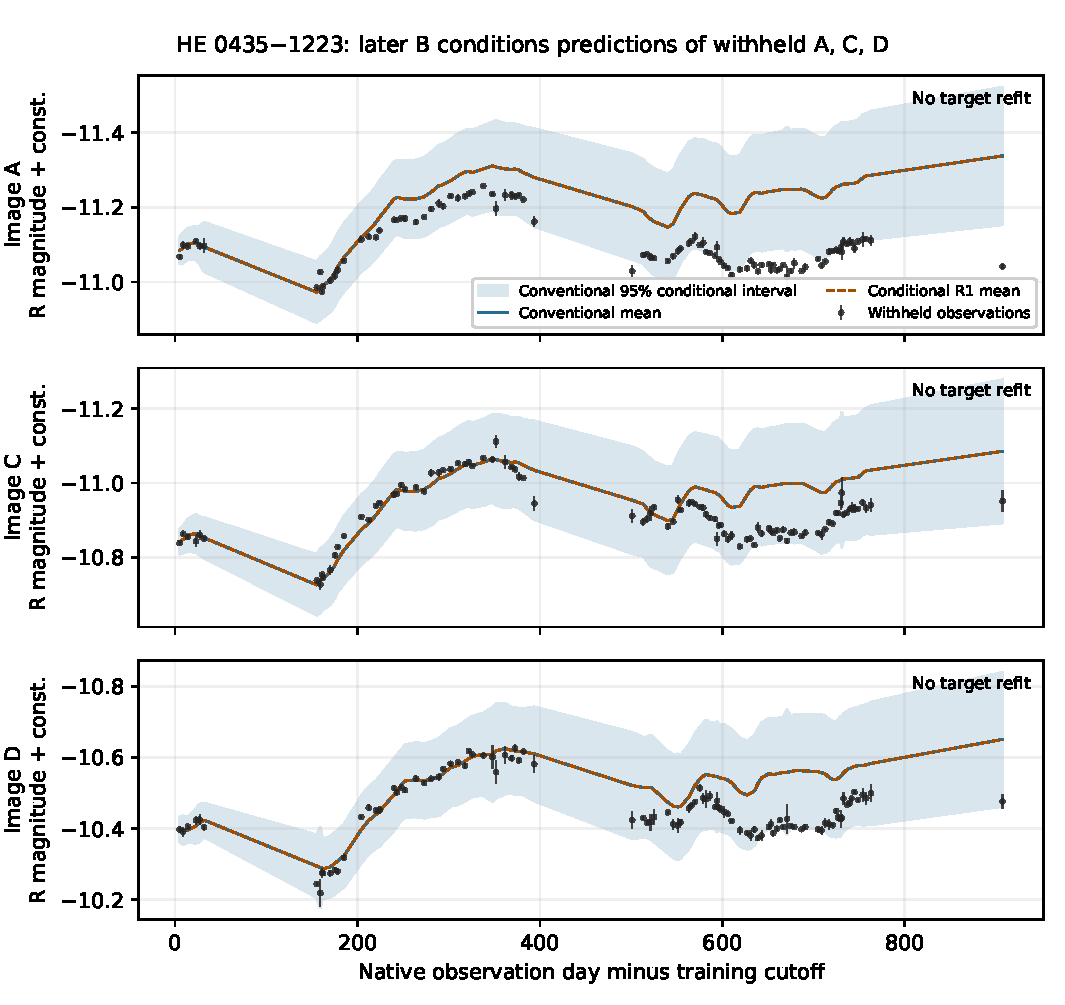
\includegraphics[width=0.96\textwidth]{figures/he0435_withheld_prediction.pdf}
 \caption{Reserved HE~0435$-$1223 A/C/D magnitudes and predictions
 conditioned on historical data and the allowed later-B driver.
 Lines join frozen predictive means at observation times; shading is
 the conventional 95\% point-parameter conditional interval. No target
 fit or per-image magnitude correction is applied. Photometry:
 COSMOGRAIL/CDS~\cite{Millon2020COSMOGRAIL}.}
 \label{fig:observed-heldout}
\end{figure}

Observed interval coverage is below nominal: conventional image-A
coverage is $62\%$, versus $99\%$ for C and $95\%$ for D. The shared
free-delay baseline also undercovers A. This is a limitation of the
brightness/uncertainty baseline, rather than a BHSM-specific residual.
The all-channel forecast has RMSE $0.194945$ mag and $75.5\%$ coverage;
the R1-minus-conventional log-score difference is again only $0.00501$.
These two factorizations use the same later observations and are not
independent replications.
Temporally correlated targets do not justify an independent-binomial
significance calculation for these coverage fractions. The model is not
retuned after this exposure; a revised variability model needs fresh
reserved data for an independent test.

A broad stationary-image search, with original-projection refinement,
finds five images in both models, including a central image with macro
flux approximately $6.32\%$ of A before microlensing, extinction and
galaxy-light contamination. No measured central-image limit enters the
point-astrometry fit. Consequently this application is a restricted
timing/point-geometry baseline, not a complete observed galaxy or
Einstein-ring reconstruction. A full imaging likelihood must test that
additional prediction. Neither its existence nor the held-out brightness
residuals are silently absorbed into a new envelope response.
